\documentclass[t]{beamer} %<- 'c' is default option, 't' forces top aligned
\usepackage[italian]{babel}
\usepackage[utf8]{inputenc}
\usepackage{graphicx,hyperref,ru,url}
\usepackage{pgf}
\usepackage{xcolor}
\usepackage{pifont}

% pacchetto per l'inclusione di figure postscript
\usepackage{graphics}
\DeclareGraphicsExtensions{.gif,.png,.pdf,.jpg,.mps}

% pacchetto per inserire figure affiancate
\usepackage{subfigure}
\usepackage[centerlast, bf]{caption}

\setbeamerfont{frametitle}{size=\large}

%Inserimento nell'indice dei numeri per ogni frame nella sezione e sottosezione 
\setbeamertemplate{section in toc}{\hspace*{1em}\inserttocsectionnumber.~\inserttocsection\par}
\setbeamertemplate{subsection in toc}{\hspace*{2em}\inserttocsectionnumber.\inserttocsubsectionnumber.~\inserttocsubsection\par}

%Ridefinizione dei comandi 
\newcommand{\virgolette}[1]{``#1''}

%Pacchetto per giustificare gli itemize
\usepackage{ragged2e}
\let\olditem=\item%
\renewcommand{\item}{\olditem \justifying}%

%Giustifica i frame
\justifying

%Pacchetto e impostazioni per i link web
\usepackage{hyperref}
\hypersetup {colorlinks=false,linkcolor=blue,filecolor=green,urlcolor=black,citecolor=blue }

% The title of the presentation:
%  - first a short version which is visible at the bottom of each slide;
%  - second the full title shown on the title slide;
\title[Prof. Orazio Tomarchio]{\LARGE Facolt\`a di Ingegneria - Universit\`a di Catania}

% Optional: a subtitle to be dispalyed on the title slide
\subtitle{
\Large Smart Intelligent University Communications \\
\Large  Software Engineering Projects\\
}
% The author(s) of the presentation:
%  - again first a short version to be displayed at the bottom;
%  - next the full list of authors, which may include contact information;
\author[Russo, Invincibile, Didomenico]
{\hspace{1.5cm} Relatore         \hspace{5.0cm} Studenti \\
\textbf {Prof. Orazio Tomarchio} \hspace{2.5cm} \textbf{Russo Leandro} \\
\hspace{6.3cm} \textbf{Invincibile Daniele} \\
\hspace{6.2cm} \textbf{Didomenico Nicola} \\
%\vspace{0.5cm}
}

% The institute:
%  - to start the name of the university as displayed on the top of each slide
%    this can be adjusted such that you can also create a Dutch version
%  - next the institute information as displayed on the title slide
\institute[Universit\`a di Catania]{
  Dipartimento di Ingegneria Elettrica, Elettronica e Informatica -- DIEEI \\
  Facolt\`a di Ingegneria Informatica}

% Add a date and possibly the name of the event to the slides
%  - again first a short version to be shown at the bottom of each slide
%  - second the full date and event name for the title slide
\date[27 Febbraio 2015]{27 Febbraio 2015}

\begin{document}

\begin{frame}
  \titlepage
\end{frame}

% Section titles are shown in at the top of the slides with the current section 
% highlighted. Note that the number of sections determines the size of the top 
% bar, and hence the university name and logo. If you do not add any sections 
% they will not be visible.

% Eliminare numeri allowframebreaks
\setbeamertemplate{frametitle continuation}{}

\section{Indice}
 \begin{frame}[allowframebreaks]{Indice} %--> oppure per il titolo del frame \frametitle {Indice}
    \tableofcontents
 \end{frame}

\section{Ideazione - Iterazione 1}
 \begin{frame}[allowframebreaks] 
  \frametitle {Descrizione realtà d'interesse} 
   Nel Piano Nazionale della Ricerca (PNR)  messo a punto da HORIZON ITALIA e MIUR viene bandito un progetto chiamato:\newline
   \textbf{\virgolette{Smart Intelligent University Communications (SIUC)}} destinato a tutti gli atenei italiani.\newline 
   Tale progetto è caratterizzato dalle seguenti specifiche descritti nel seguito, che consente ad appassionati, studenti,    
   ricercatori, docenti e imprese di scambiarsi messaggi in tempo reale su condivisioni, integrazioni e competenze di idee per una contaminazione tra ambiti 
   disciplinari diversi, realtà diverse e stimolare nei partecipanti lo sviluppo della  cultura dell’intraprendere e dell’innovazione.\newline 
   In tale sistema si richiedono le seguenti specifiche:
   \begin{itemize} 
    \item Esistono diversi canali o stanze virtuali (ciascuna legata a un corso di laurea per ogni facoltà, includendo sia la triennale e la magistrale di quel 
          determinato corso di laurea) nelle quali un utente può entrare per scambiare messaggi con gli altri utenti presenti nella stessa stanza.
    \item \`E possibile inviare due tipi di messaggi: 
          \setbeamertemplate{itemize items}[triangle]
          \begin{itemize} 
            \item \virgolette{pubblici}: dei messaggi inviati da un utente e trasmessi a tutti gli altri partecipanti presenti nella stanza; 
            \item \virgolette{privati}: dei messaggi inviati da un utente e trasmessi ad uno specifico partecipante presente nella stessa stanza, in questo caso il 
                                        destinatario selezionato sarà l’unico a ricevere il messaggio.
          \end{itemize}
          \setbeamertemplate{itemize items}[circle]
    \item In ogni istante il sistema prevede la presenza di una tipologia di utente particolare, chiamato amministratore. I compiti più importanti di un 
          amministratore sono i seguenti: 
          \setbeamertemplate{itemize items}[triangle]
          \begin{itemize} 
            \item può creare o eliminare stanze del servizio di messaggistica; 
            \item inviare messaggi di avviso ad un utente;
            \item in caso di comportamenti irregolari è possibile espellere un utente dalla stanza e l'utente non può più rientrare fin quando questo non sarà
                  rimosso dalla lista dei partecipanti bannati della stanza presente nel sistema.
          \end{itemize}
    \item Il sistema deve mandare dei messaggi di notifica, che permettono di aggiornare l’utente di un cambiamento dello stato del sistema.
  \end{itemize}
\end{frame}

\subsection{Iterazione 1: Requisiti}
\begin{frame} [allowframebreaks]
  \frametitle{Iterazione 1: Requisiti - Documento di Visione}
   La caratteristica principale del progetto è quella di consentire ad appassionati, studenti, ricercatori, docenti e imprese di scambiarsi messaggi in tempo reale   
   per ogni ateneo.  In particolare in questo progetto sono presenti diverse stanze virtuali che rappresentano le facoltà di un ateneo con due tipologie di    
   utilizzatori di sistema, ovvero l’amministratore e gli utenti del servizio di messaggistica.  Con le seguenti  caratteristiche:
   \begin{itemize} 
    \item l’amministratore gestisce le stanze virtuali e supervisiona gli utenti del servizio;
    \item gli utenti per usufruire di tale servizio inseriscono un nickname e si collegano al server impostando dei parametri di connessione. Ogni utente può    
          accedere a una stanza e inviare messaggi ad ogni utente presente nella stanza in tempo reale, inoltre ognuno può contattare in maniera privata gli altri 
          partecipanti presenti nella stanza.
   \end{itemize}
   L’architettura utilizzata per offrire il servizio è di tipo client-server, questo approccio consente di fornire un’interfaccia  più flessibile per l’accesso al   
   servizio di messaggistica anche con un semplice browser, senza modificare pesantemente la progettazione rispetto ad un architettura peer-to-peer.
\end{frame}

\begin{frame}
  \frametitle{Iterazione 1: Requisiti - Diagrammi dei casi d'uso}
    \hypersetup{linkbordercolor={0 0.5 0.1}}
    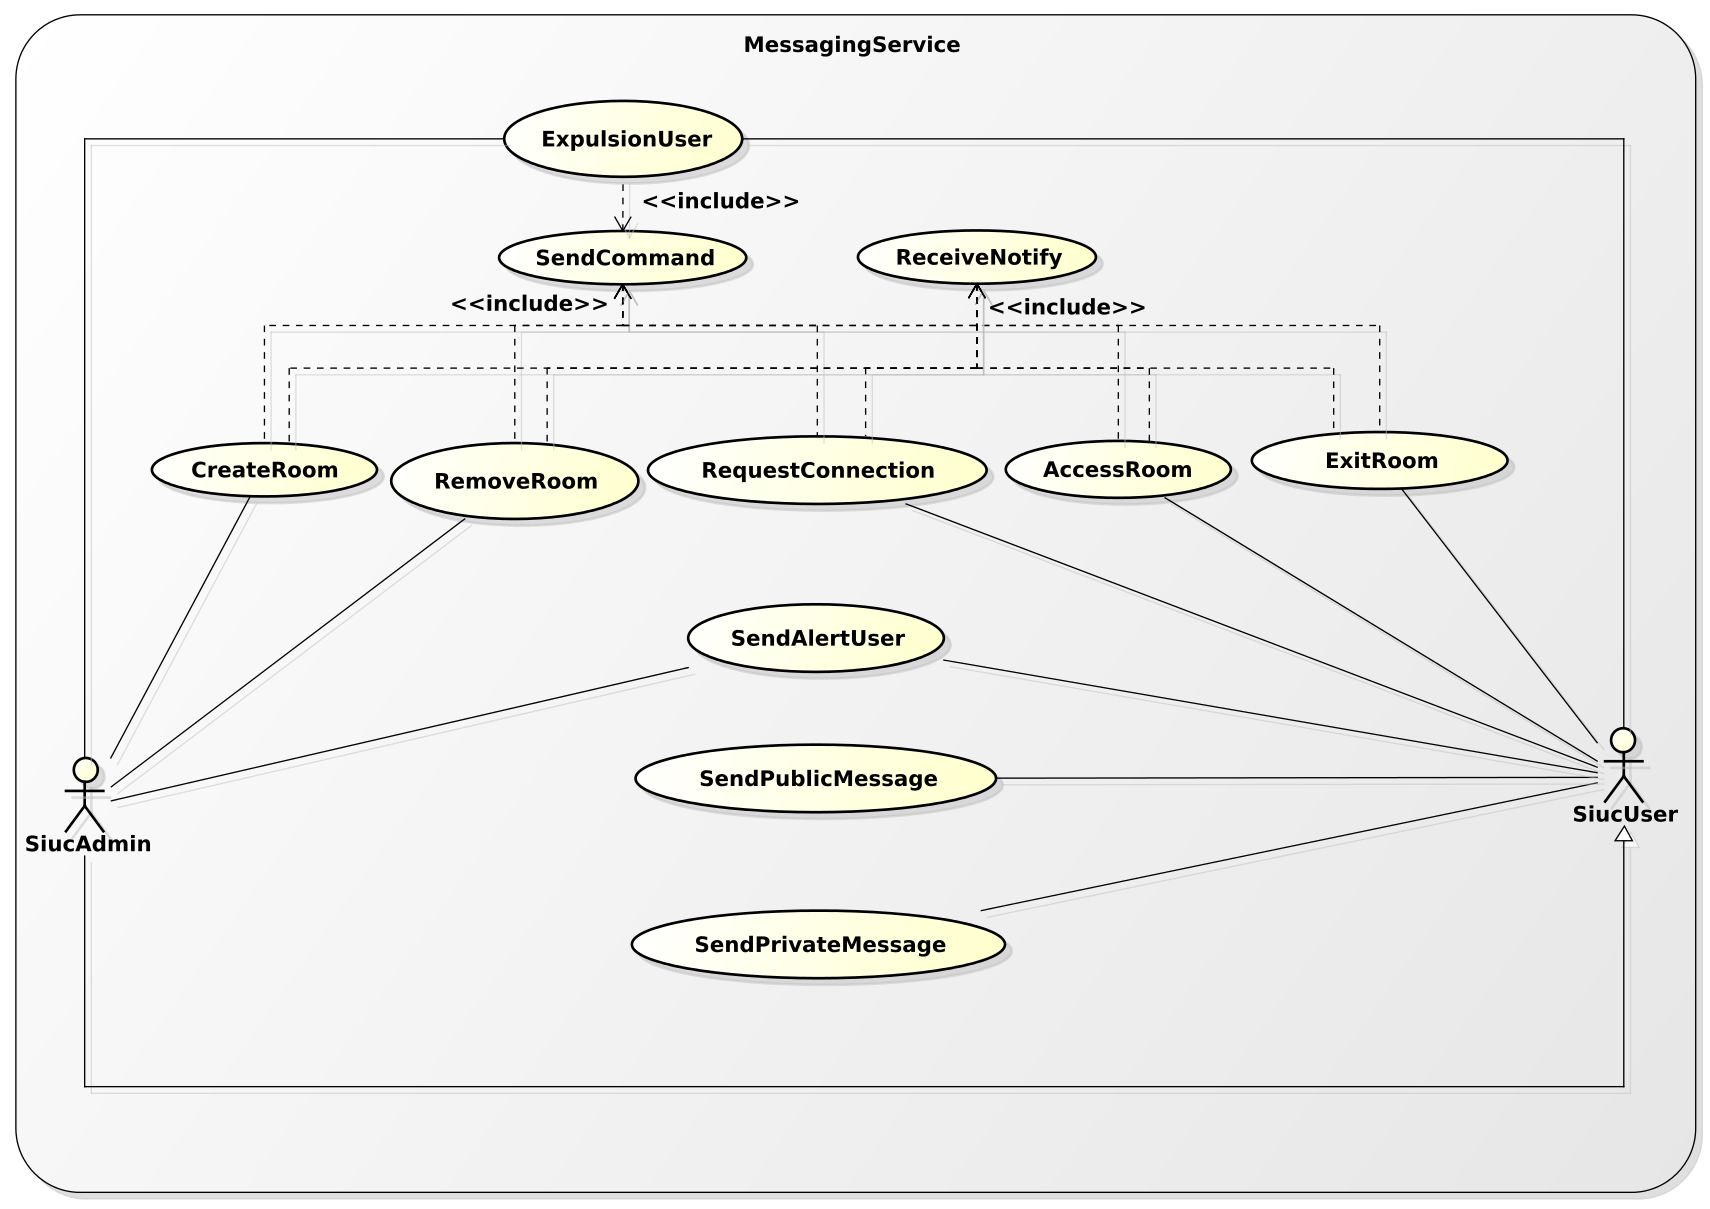
\includegraphics[height=178px, width=330px,]{image_astah/UseCaseDiagram.png}{\centering}
\end{frame}

\begin{frame} [allowframebreaks]
  \frametitle{Iterazione 1: Requisiti - Modello dei casi d'uso}
   \underline{Attori Identificati}: Amministratore (SiucAdmin) e Utente del Servizio di Messaggistica (SiucUser). \newline
   \underline{Casi d'uso identificati}: RequestConnection, AccessRoom, SendRoomMessage, SendPrivateMessage, ReceiveNotify, ExitRoom, CreateRoom, RemoveRoom, 
                                        SendAlertUser, ExpulsionUser \newline
   Descrizione breve dei casi d'uso identificati:
   \begin{enumerate} 
    \item RequestConnection. L’utente si connette al sistema specificando il nickname, l’indirizzo e la porta del servizio di messaggistica.
    \item AccessRoom. L’utente richiede al sistema l’ingresso in una specifica stanza del servizio (che deve essere stata precedentemente creata dall’amministratore 
          del servizio). 
    \item SendRoomMessage. Il partecipante al servizio di messaggistica invia un messaggio ``pubblico'' che viene inviato dal sistema a tutti i partecipanti che si 
          trovano nella stessa stanza di colui che ha inviato il messaggio.
    \item SendPrivateMessage. Il partecipante al servizio di messaggistica  invia un messaggio ``privato'' ad uno specifico partecipante.
    \item ReceiveNotify. Il sistema manda dei messaggi di notifica, che permettono di aggiornare l’utente di un cambiamento dello stato del sistema.
    \item ExitRoom. Un partecipante richiede al sistema l’uscita dal servizio. Questo comporta la sua eliminazione dall’insieme dei partecipanti presenti nella 
          stanza del servizio cui era precedentemente associato l’utente.
    \item CreateRoom. L’amministratore del servizio di messaggistica è responsabile della creazione (preventiva) delle stanze che potranno successivamente essere 
          visitate dai partecipanti.
    \item RemoveRoom. In ogni momento l’amministratore può eliminare una stanza dal servizio (ad esempio perchè non ci sono partecipanti). Ciò comporta l’invio 
          preventivo di un messaggio a tutti i patecipanti eventualmente presenti nella stanza, i quali potranno in seguito richiedere l’ingresso in una   
          nuova stanza del servizio.
    \item SendAlertUser. L’amministratore può in ogni momento inviare un messaggio di avviso ad uno specifico partecipante al servizio.
    \item ExpulsionUser. L’amministratore può in ogni momento espellere da una stanza uno specifico partecipante.  
   \end{enumerate}
\end{frame}

\begin{frame}
 \frametitle{Iterazione 1: Requisiti, caso d'uso UC1\_RequestConnection}
  \begin{table}[!htbp]
    \caption {Descrizione Dettagliata: Caso d'uso UC1\_RequestConnection}
    \label{table:1}
     \resizebox{\linewidth}{!}{%
      \begin{tabular}{|l|p{10cm}|}\hline
       Nome caso d'uso &  UC1\_RequestConnection \\\hline
       Portata & Applicazione Smart Intelligent University Communications \\\hline
       Livello &  Obiettivo Utente \\\hline
       Attore primario &  SiucUser \\\hline
       Parti interessate e interessi &  SiucUser: vuole collegarsi al servizio di messaggistica \\\hline
       Pre-condizioni & L'utente ha bisogno di una connessione di rete\\\hline
       Post-condizioni (garanzia di successo) &  L'utente è inserito tra gli utenti online con il nickname confermato dal servizio di messaggistica ottenendo un 
                                                 messaggio di benvenuto \\\hline
       Scenario principale di successo &  
       \begin{enumerate} 
       \item L'utente inserisci un nickname, l'address e la porta del server.
       \item Il sistema esamina il nickname inviato dall'utente e verifica se è presente una omonimia.
       \item Il sistema conferma l'inserimento tra gli utenti online inviando una notifica di benvenuto.
       \end{enumerate} \\\hline
      \end{tabular}}
   \end{table}
\end{frame}

\begin{frame}
 \frametitle{Iterazione 1: Requisiti, caso d'uso UC1\_RequestConnection}
  \begin{table}[!htbp]
      \resizebox{\linewidth}{!}{%
       \begin{tabular}{|l|p{10cm}|}\hline
         Estensioni (o flussi alternativi) &  
           1A - SiucUser inserisce parametri errati: 
          \begin{itemize} 
           \item Viene visualizzato un messaggio di errore e viene richiesto nuovamente l’inserimento di tali parametri.
          \end{itemize} 
           2A - Omonimia del nickname:
          \begin{itemize}       
           \item Il sistema cambia il nickname aggiungendo "\_" al nickname (es. \_nickname). 
           \item Il sistema conferma l'inserimento tra gli utenti online inviando una notifica di benvenuto.
          \end{itemize} \\\hline
       Requisiti speciali (Requisiti Non Funzionali) &  Comunicazione asincrona in cui lo scambio di informazioni avviene in tempo reale, senza sensibili pause tra 
                                                        invio e ricezione del messaggio.\\\hline
       Elenco delle varianti tecnologiche &  L’applicazione dovrebbe essere flessibile al funzionamento di diversi protocolli di comunicazione (es. TCP, UDP) e con   
       diversi strati middleware (es. Socket, RMI) \\\hline
       Frequenza di ripetizione & Potrebbe essere quasi ininterrotta \\\hline
       Varie e/o Problemi Aperti &  // \\\hline
      \end{tabular}}
   \end{table}
\end{frame}

\begin{frame}
 \frametitle{Iterazione 1: Requisiti, caso d'uso UC2\_AccessRoom}
  \begin{table}[!htbp]
   \caption {Caso d'uso UC2\_AccessRoom}
    \label{table:1}
     \resizebox{\linewidth}{!}{%
      \begin{tabular}{|l|p{10cm}|}\hline
       Nome caso d'uso &  UC2\_AccessRoom\\\hline
       Portata & Applicazione Smart Intelligent University Communications \\\hline
       Livello & Obiettivo Utente \\\hline
       Attore primario & SiucUser  \\\hline
       Parti interessate e interessi & SiucUser: vuole registrarsi e effettuare l’ingresso in una stanza presente nel servizio di messaggistica \\\hline
       Pre-condizioni & Nel sistema è presente almeno una stanza creata da un amministratore.\\\hline
       Post-condizioni (garanzia di successo) &  Nel caso di svolgimento normale l’utente è registrato ed è presente nell’insieme degli utenti della stanza 
                                                 specificata. \\\hline
      \end{tabular}}
   \end{table}
\end{frame}

\begin{frame}
 \frametitle{Iterazione 1: Requisiti, caso d'uso UC2\_AccessRoom}
  \begin{table}[!htbp]
      \resizebox{\linewidth}{!}{%
       \begin{tabular}{|l|p{10cm}|}\hline
          Scenario principale di successo &  
           \begin{enumerate} 
            \item L’utente richiede una lista di stanze presenti nel sistema  di messaggistica.
            \item Il sistema invia la lista delle stanze.
            \item L’utente seleziona la stanza tra quelle presenti in lista.
            \item Il sistema registra l’utente alla stanza.
          \end{enumerate} \\\hline 
         Estensioni (o flussi alternativi) &  
           3A - Il SiucUser inserisce una stanza non in elenco:
          \begin{enumerate} 
           \item Il sistema invia un messaggio di errore.
          \end{enumerate} \\\hline
       Requisiti speciali (Requisiti Non Funzionali) &  Comunicazione asincrona in cui lo scambio di informazioni avviene in tempo reale, senza sensibili pause tra 
                                                        invio e ricezione del messaggio.\\\hline
       Elenco delle varianti tecnologiche &  L’applicazione dovrebbe essere flessibile al funzionamento di diversi protocolli di comunicazione (es. TCP, UDP) e con   
       diversi strati middleware (es. Socket, RMI) \\\hline
       Frequenza di ripetizione & Potrebbe essere quasi ininterrotta \\\hline
       Varie e/o Problemi Aperti &  // \\\hline
      \end{tabular}}
   \end{table}
\end{frame}

\begin{frame}
 \frametitle{Iterazione 1: Requisiti, Mockups Bozza User Interface}
    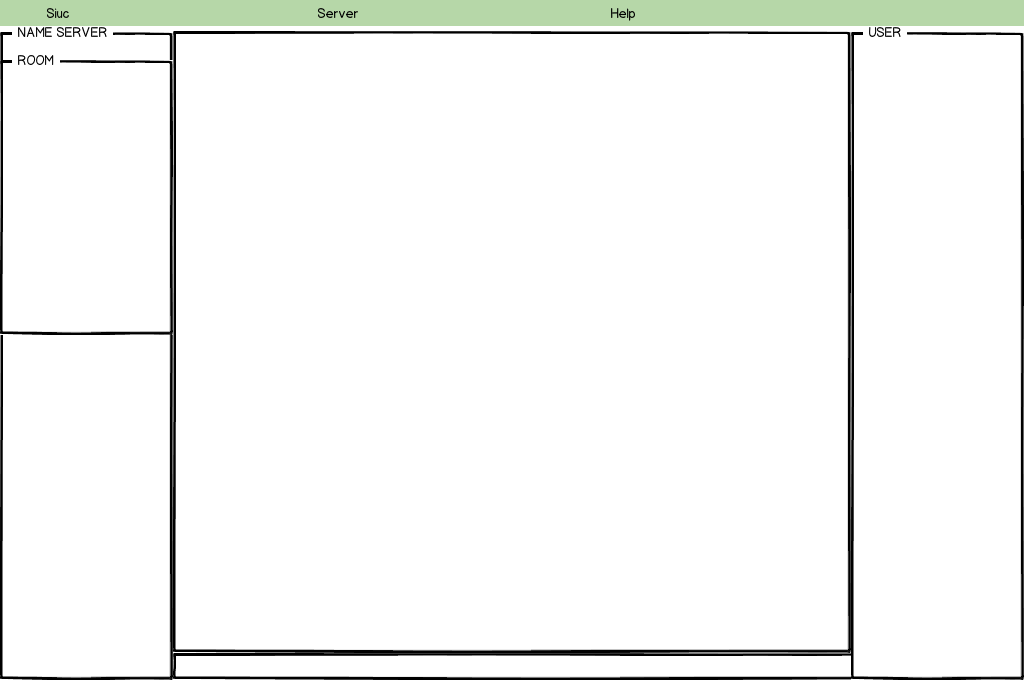
\includegraphics[height=190px, width=286px,]{image_mockups/01_siuc_open.png}{\centering}
\end{frame}

\begin{frame}
 \frametitle{Iterazione 1: Requisiti, Mockups Bozza User Interface}
    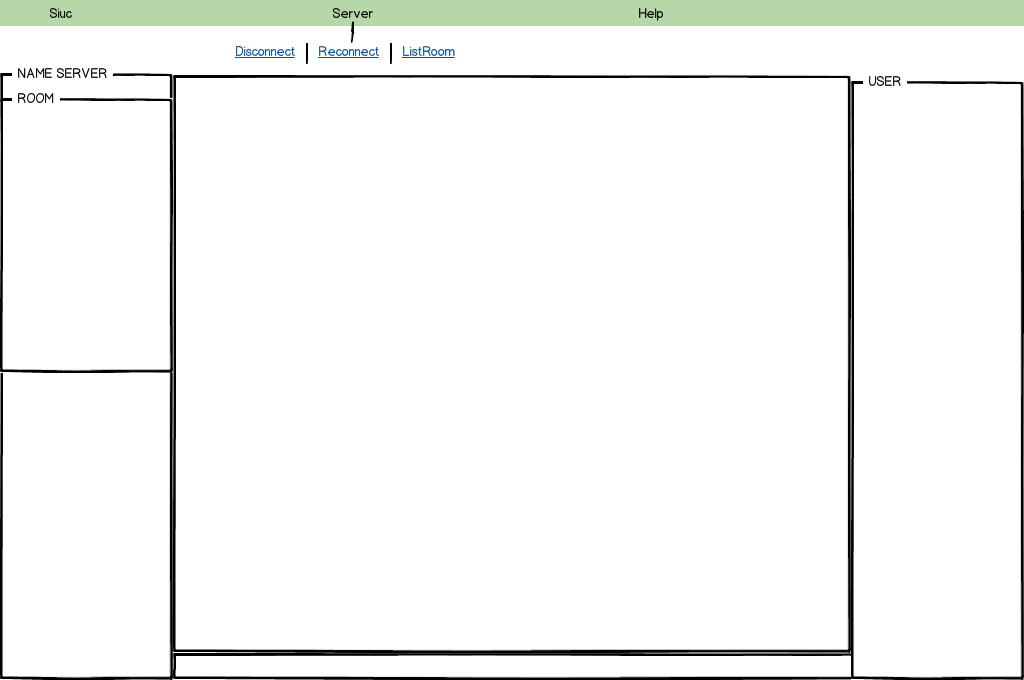
\includegraphics[height=190px, width=286px,]{image_mockups/02_siuc_menu_server.png}{\centering}
\end{frame}

\begin{frame}
 \frametitle{Iterazione 1: Requisiti, Mockups Bozza User Interface}
    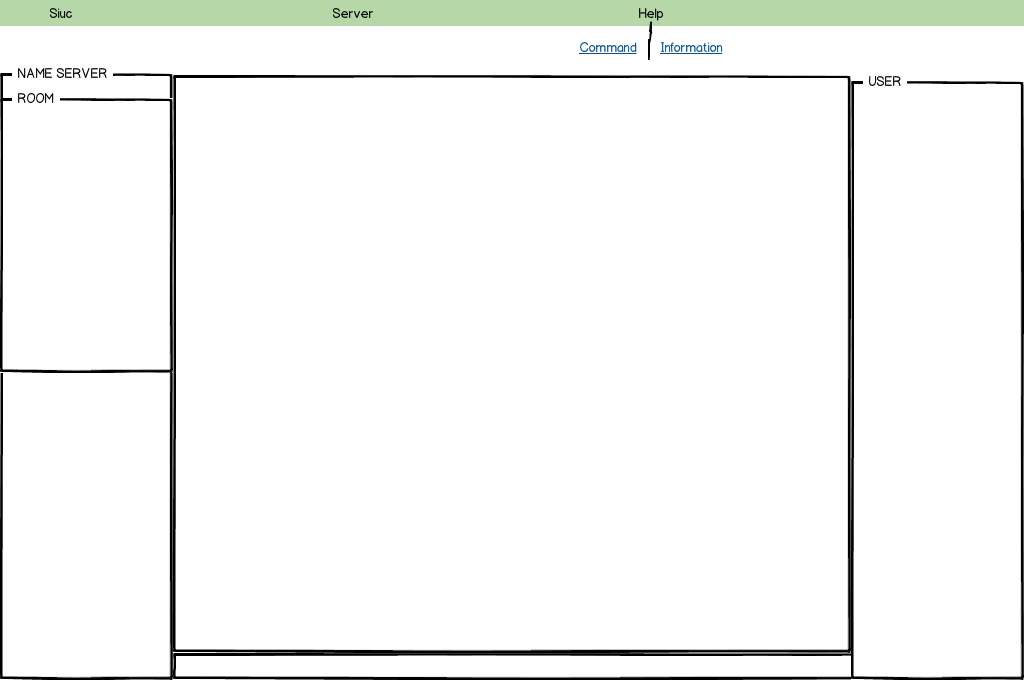
\includegraphics[height=190px, width=286px,]{image_mockups/03_siuc_menu_help.png}{\centering}
\end{frame}

\begin{frame}
 \frametitle{Iterazione 1: Requisiti, Mockups Bozza User Interface}
    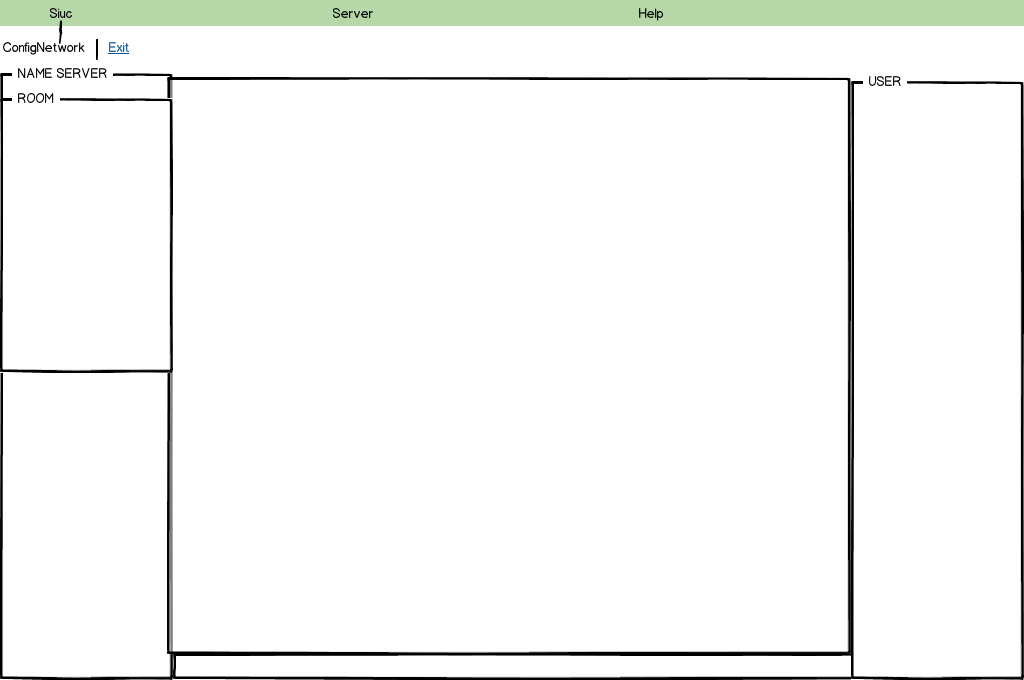
\includegraphics[height=190px, width=286px,]{image_mockups/04_siuc_menu_siuc.png}{\centering}
\end{frame}

\begin{frame}
 \frametitle{Iterazione 1: Requisiti, Mockups Bozza User Interface}
    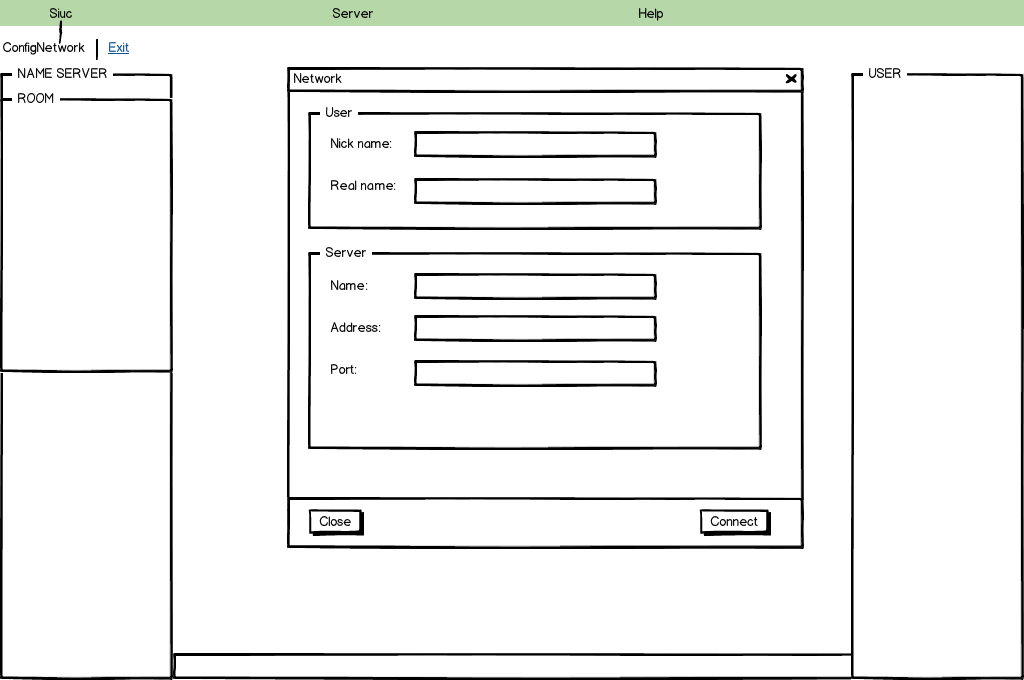
\includegraphics[height=190px, width=286px,]{image_mockups/05_siuc_config_network.png}{\centering}
\end{frame}

\begin{frame}
 \frametitle{Iterazione 1: Requisiti, Mockups Bozza User Interface}
    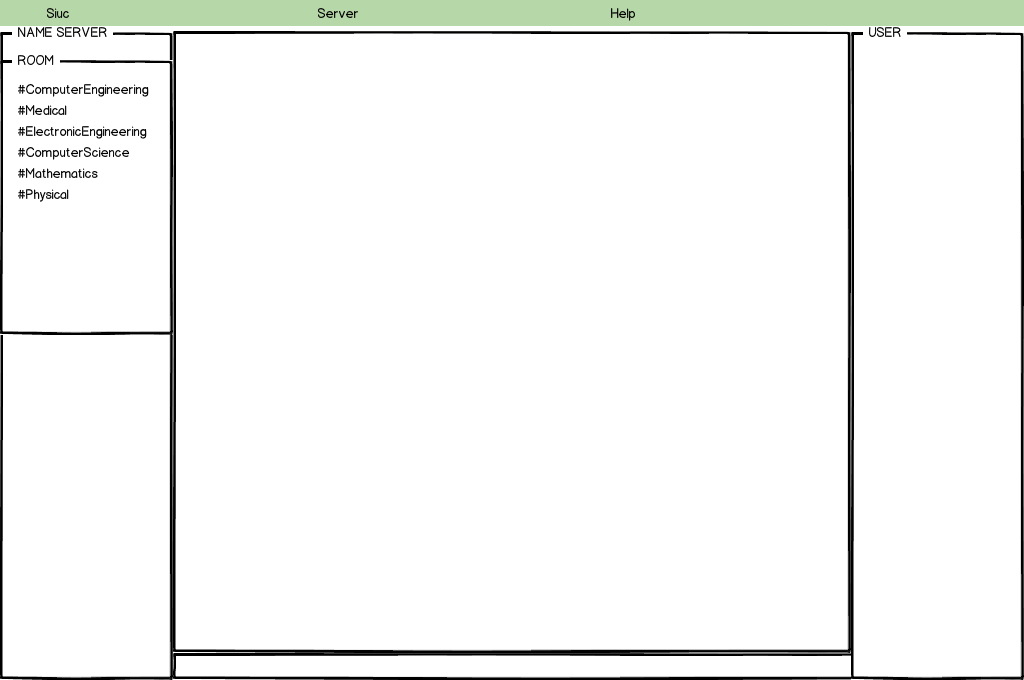
\includegraphics[height=190px, width=286px,]{image_mockups/06_siuc_connect.png}{\centering}
\end{frame}

\begin{frame}
 \frametitle{Iterazione 1: Requisiti, Mockups Bozza User Interface}
    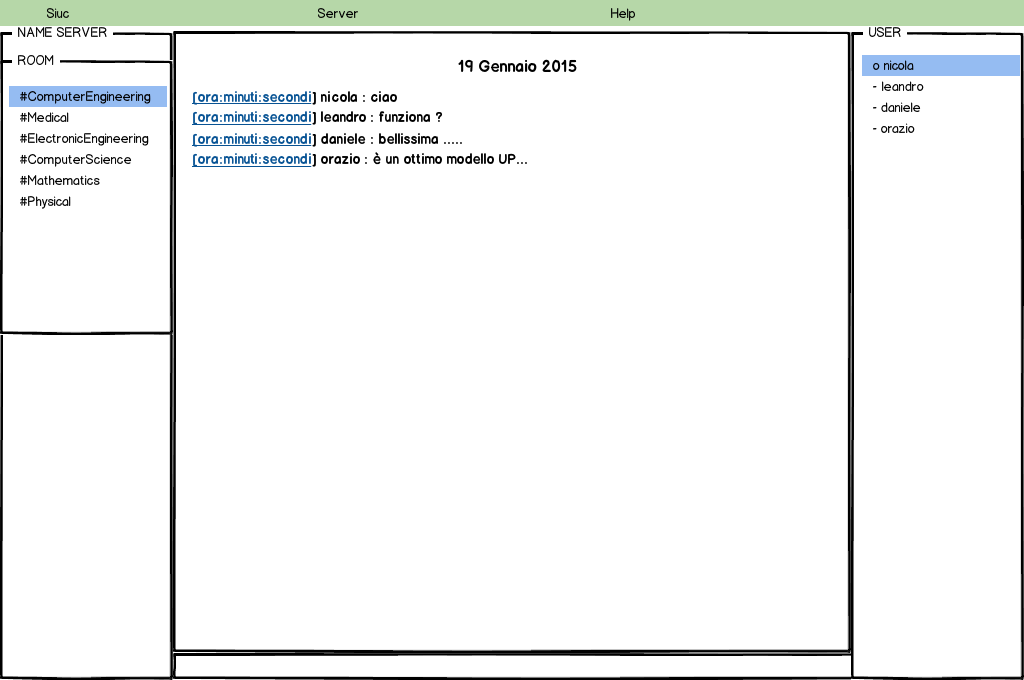
\includegraphics[height=190px, width=286px,]{image_mockups/07_siuc_user_room_ce.png}{\centering}
\end{frame}

\begin{frame}
 \frametitle{Iterazione 1: Requisiti, Mockups Bozza User Interface}
    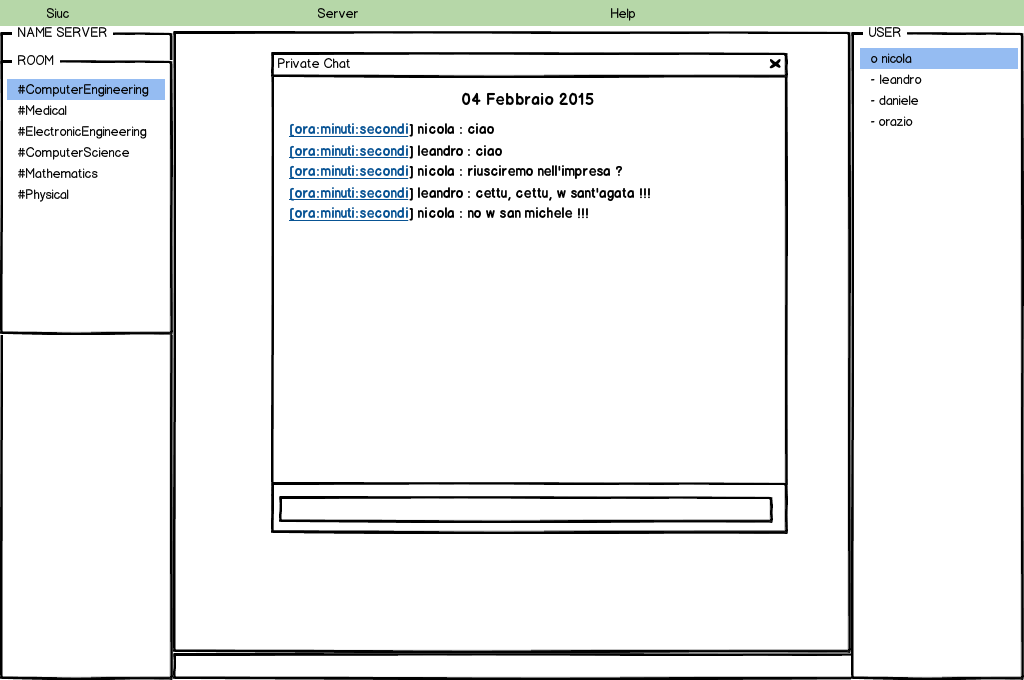
\includegraphics[height=190px, width=286px,]{image_mockups/08_siuc_user_room_ce_private.png}{\centering}
\end{frame}

\begin{frame}
 \frametitle{Iterazione 1: Requisiti, Mockups Bozza User Interface}
    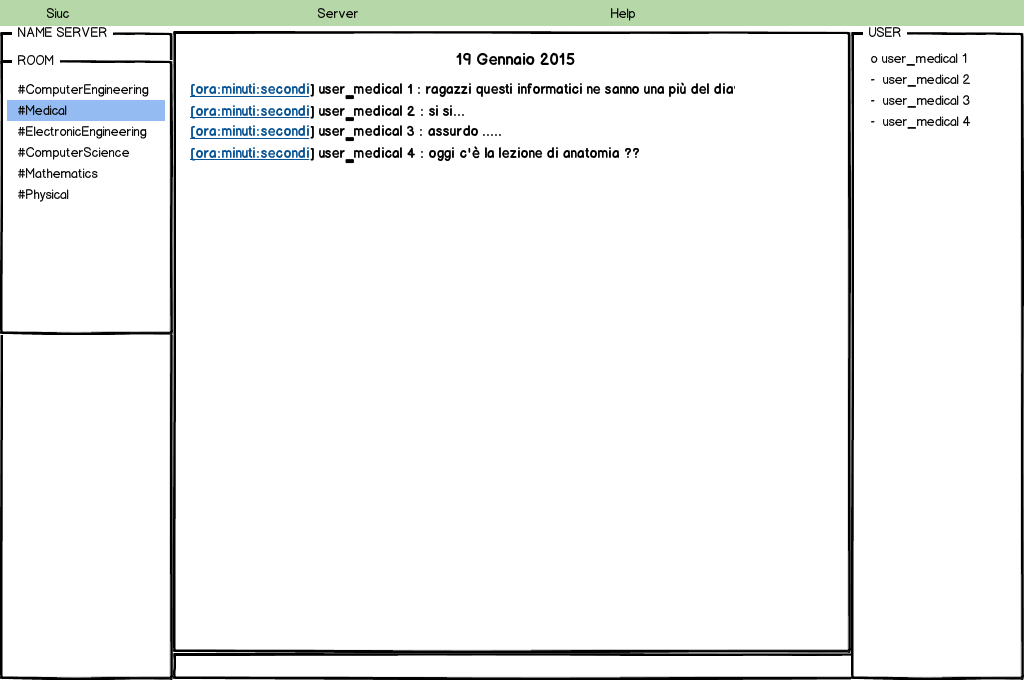
\includegraphics[height=190px, width=286px,]{image_mockups/09_siuc_user_room_medical.png}{\centering}
\end{frame}

\subsection{Iterazione 1: Analisi, casi d'uso UC1 e UC2}
\begin{frame} {Iterazione 1: Analisi, casi d'uso UC1 e UC2}
\end{frame}

\begin{frame}
 \frametitle{Iterazione 1: Analisi, contratto CO1 - nameCO1}
  \begin{table}[!htbp]
   \caption {Contratto CO1 - nameCO1}
    \label{table:1}
      \resizebox{\linewidth}{!}{%
       \begin{tabular}{|l|p{10cm}|}\hline
         Operazione & \\\hline 
         Riferimenti &  \\\hline
         Pre-condizione & \\\hline 
         Post-condizione &  \\\hline
      \end{tabular}}
   \end{table}
\end{frame}

\subsection{Iterazione 1: Progettazione}
\begin{frame}
 \frametitle{Iterazione 1: Progettazione, casi d'uso UC1 e UC2}
\end{frame}

\subsection{Iterazione 1: Implementazione}
\begin{frame}
 \frametitle{Iterazione 1: Implementazione, casi d'uso UC1 e UC2}
\end{frame}

\subsection{Iterazione 1: Test}
\begin{frame}
 \frametitle{Iterazione 1: Test, casi d'uso UC1 e UC2}
\end{frame}

\section{Ideazione - Refactoring}
\begin{frame}
  \frametitle{Descrizione Iterazione 1 con Refactoring}
\end{frame}

\subsection{Iterazione 1 - Refactoring: Progettazione}
\begin{frame}
  \frametitle{Iterazione 1 - Refactoring: Progettazione, casi d'uso UC1 e UC2}
\end{frame}

\subsection{Iterazione 1 - Refactoring: Implementazione}
\begin{frame}
  \frametitle{Iterazione 1 - Refactoring: Implementazione, casi d'uso UC1 e UC2}
\end{frame}

\subsection{Iterazione 1 - Refactoring: Test}
\begin{frame}
  \frametitle{Iterazione 1 - Refactoring: Test, casi d'uso UC1 e UC2}
\end{frame}

\section{Elaborazione - Iterazione 2}
\begin{frame}
  \frametitle{Descrizione Iterazione 2}
\end{frame}

\subsection{Iterazione 2: Requisiti}
\begin{frame}
  \frametitle{Iterazione 2: Requisiti, caso d'uso UC3\_SendRoomMessage}
  \begin{table}[!htbp]
    \caption {Caso d'uso UC3\_SendRoomMessage}
     \label{table:1}
      \resizebox{\linewidth}{!}{%
       \begin{tabular}{|l|p{10cm}|}\hline
        Nome caso d'uso &  UC3\_SendRoomMessage\\\hline
        Portata & Applicazione Smart Intelligent University Communications \\\hline
        Livello & Obiettivo Utente \\\hline
        Attore primario & SiucUser  \\\hline
        Parti interessate e interessi & 
         \begin{itemize}
          \item SiucUser, vuole che i messaggi siano inviati a ogni utente della stanza virtuale.
          \item SiucAdmin, è interessato a supervisionare gli utenti del servizio affinché non ci siano abusi.       
         \end{itemize} \\\hline
        Pre-condizioni &  L'utente è registrato nella stanza in cui desidera inviare i messaggi.\\\hline
        Post-condizioni (garanzia di successo) & Ogni utente riceve il messaggio inviato. \\\hline
      \end{tabular}}
   \end{table}
\end{frame}

\begin{frame}
 \frametitle{Iterazione 2: Requisiti, caso d'uso UC3\_SendRoomMessage}
  \begin{table}[!htbp]
      \resizebox{\linewidth}{!}{%
       \begin{tabular}{|l|p{10cm}|}\hline
         Scenario principale di successo &  
         \begin{enumerate} 
          \item Il sistema visualizza a video gli utenti presenti nella stanza.
          \item Il sistema visualizza un’area pubblica dove vengono mostrati tutte le conversazioni in corso dal quel momento in poi. 
          \item L’utente inserisce da tastiera il messaggio da inviare.
          \item Il messaggio viene inoltrato agli altri utenti presenti nella stanza selezionata. 
         \end{enumerate} \\\hline
         Estensioni (o flussi alternativi) &  
           1A - La connessione fallisce:
          \begin{itemize} 
           \item Il server rimuove l’utente dalle stanze in cui è registrato.
          \end{itemize} \\\hline
         Requisiti speciali (Requisiti Non Funzionali) &  Comunicazione asincrona in cui lo scambio di informazioni avviene in tempo reale, senza sensibili pause tra 
                                                        invio e ricezione del messaggio\\\hline
      \end{tabular}}
   \end{table}
\end{frame}

\begin{frame} 
 \frametitle{Iterazione 2: Requisiti, caso d'uso UC3\_SendRoomMessage}
  \begin{table}[!htbp]
      \resizebox{\linewidth}{!}{%
       \begin{tabular}{|l|p{10cm}|}\hline
         Elenco delle varianti tecnologiche &  
          \begin{itemize}  
           \item \`E possibile inviare messaggi confidenziali, autenticati e integri al server del servizio di messaggistica.
           \item L’applicazione dovrebbe essere flessibile al funzionamento di diversi protocolli di comunicazione (es. TCP, UDP) e con diversi strati middleware 
                 (es. Socket, RMI)
          \end{itemize} \\\hline
         Frequenza di ripetizione & Potrebbe essere quasi ininterrotta \\\hline
         Varie e/o Problemi Aperti &  // \\\hline
      \end{tabular}}
   \end{table}
\end{frame}

\subsection{Iterazione 2: Analisi}
\begin{frame}
  \frametitle{Iterazione 2: Analisi, caso d'uso UC3\_SendRoomMessage}
\end{frame}

\subsection{Iterazione 2: Progettazione}
\begin{frame}
  \frametitle{Iterazione 2: Progettazione, caso d'uso UC3\_SendRoomMessage}
\end{frame}

\subsection{Iterazione 2: Implementazione}
\begin{frame}
  \frametitle{Iterazione 2: Implementazione, caso d'uso UC3\_SendRoomMessage}
\end{frame}

\subsection{Iterazione 2: Test}
\begin{frame}
  \frametitle{Iterazione 2: Test, caso d'uso UC3\_SendRoomMessage}
\end{frame}

\section{Elaborazione - Iterazione 3}
\begin{frame}
  \frametitle{Descrizione Iterazione 3}
\end{frame}

\subsection{Iterazione 3: Requisiti}
\begin{frame}
  \frametitle{Iterazione 3: Requisiti, caso d'uso UC4\_SendPrivateMessage}
  \begin{table}[!htbp]
    \caption {Caso d'uso UC4\_SendPrivateMessage}
     \label{table:1}
      \resizebox{\linewidth}{!}{%
       \begin{tabular}{|l|p{10cm}|}\hline
        Nome caso d'uso &  UC4\_SendPrivateMessage\\\hline
        Portata & Applicazione Smart Intelligent University Communications \\\hline
        Livello & Obiettivo Utente \\\hline
        Attore primario & SiucUser  \\\hline
        Parti interessate e interessi & 
         \begin{itemize}
          \item SiucUser: vuole che i messaggi siano inviati all’utente selezionato presente nella stanza virtuale.      
         \end{itemize} \\\hline
        Pre-condizioni &
         \begin{itemize}  
          \item L'utente è registrato nella stanza in cui desidera inviare un messaggio ad un altro utente presente.
         \end{itemize} \\\hline
        Post-condizioni (garanzia di successo) &  L’utente selezionato riceve il messaggio inviato\\\hline
      \end{tabular}}
   \end{table}
\end{frame}

\begin{frame}
 \frametitle{Iterazione 3: Requisiti, caso d'uso UC4\_SendPrivateMessage}
  \begin{table}[!htbp]
      \resizebox{\linewidth}{!}{%
       \begin{tabular}{|l|p{10cm}|}\hline
         Scenario principale di successo &  
         \begin{enumerate} 
          \item L’utente seleziona una stanza.
          \item Il sistema visualizza a video gli utenti presenti nella stanza e un’area pubblica dove vengono mostrati tutte le conversazioni in corso da quel 
                momento in poi.
          \item L’utente seleziona il destinatario del messaggio privato.
          \item L’utente inserisce da tastiera il messaggio da inviare.
	  \item Il messaggio viene inoltrato al destinatario selezionato.
         \end{enumerate} \\\hline
         Estensioni (o flussi alternativi) &  
           1A - La connessione fallisce:
          \begin{itemize} 
           \item Il server rimuove l’utente dalle stanze in cui è registrato.
          \end{itemize} \\\hline
         Requisiti speciali (Requisiti Non Funzionali) &  Comunicazione asincrona in cui lo scambio di informazioni avviene in tempo reale, senza sensibili pause tra 
                                                        invio e ricezione del messaggio\\\hline
      \end{tabular}}
   \end{table}
\end{frame}

\begin{frame}
 \frametitle{Iterazione 3: Requisiti, caso d'uso UC4\_SendPrivateMessage}
  \begin{table}[!htbp]
      \resizebox{\linewidth}{!}{%
       \begin{tabular}{|l|p{10cm}|}\hline
         Elenco delle varianti tecnologiche &  
          \begin{itemize}  
           \item \`E possibile inviare messaggi confidenziali, autenticati e integri al server del servizio di messaggistica.
           \item L’applicazione dovrebbe essere flessibile al funzionamento di diversi protocolli di comunicazione (es. TCP, UDP) e con diversi strati middleware 
                 (es. Socket, RMI)
          \end{itemize} \\\hline
         Frequenza di ripetizione & Potrebbe essere quasi ininterrotta \\\hline
         Varie e/o Problemi Aperti &  // \\\hline
      \end{tabular}}
   \end{table}
\end{frame}

\subsection{Iterazione 3: Analisi}
\begin{frame}
  \frametitle{Iterazione 3: Analisi, caso d'uso UC4\_SendPrivateMessage}
\end{frame}

\subsection{Iterazione 3: Progettazione}
\begin{frame}
  \frametitle{Iterazione 3: Progettazione, caso d'uso UC4\_SendPrivateMessage}
\end{frame}

\subsection{Iterazione 3: Implementazione}
\begin{frame}
  \frametitle{Iterazione 3: Implementazione, caso d'uso UC4\_SendPrivateMessage}
\end{frame}

\subsection{Iterazione 3: Test}
\begin{frame}
  \frametitle{Iterazione 3: Test, caso d'uso UC4\_SendPrivateMessage}
\end{frame}

\section{Glossario}
\setbeamertemplate{itemize items}[triangle]
\begin{frame} [allowframebreaks]
  \frametitle{Glossario} 
   \begin{itemize} 
    \item SiucUser, User, Utente: è l'utente del servizio di messaggistica che usufruisce dei servizi forniti.
    \item SiucAdmin, Admin, Amministratore: è il gestore del servizio di messaggistica, che possiedono la facoltà di creare e/o eliminare una stanza, di inviare un 
          particolare messaggio di avviso ad un partecipante per un comportamento non corretto ed eventualmente di bannarlo eliminandolo dalla stanza.
    \item Servizio di messaggistica, sistema, (chat): ...
    \item Room, stanza, canale: insieme che si può differenziare dalle altre in base alle tematiche trattate.
    \item Comando, Comand: particolare istruzione inserita da un utente o partecipante per richiedere un determinato servizio. Vediamo qui di seguito l’elenco dei 
          comandi implementati:
     \setbeamertemplate{itemize items}[circle]
     \begin{itemize} 
      \item /listRooms:	comando che restituisce la lista delle stanze presenti nel server.
      \item /join '[nameRoom]': comando che permette la registrazione dell’utente nella stanza che ha come nome NameRoom.
     \end{itemize}   
    \item Messaggio Pubblico: messaggio testuale inviato da un partecipante a tutti gli utenti presenti nella stanza.
    \item Messaggio Privato: messaggio testuale inviato da un partecipante ad un particolare partecipante presente nella stanza.
    \item Notifica: particolari messaggi di avviso inviati dal server agli utenti del servizio.  
  \end{itemize}
\end{frame}

\begin {frame} 
 \frametitle {\refname}
  \begin {thebibliography}{99}
   {\tiny 
     \bibitem {bib1}  Martin Fowler, L. Baresi, S. Gaburri 
     \newblock \emph{UML distilled. Guida rapida al linguaggio di modellazione standard} 
     \newblock {Pearson Education Italia, 2010}

     \bibitem {bib2} Craig Larman, Luca Cabibbo
     \newblock \emph{Applicare UML e i pattern: analisi e progettazione orientata agli oggetti} 
     \newblock {Pearson Education Italia, 2005}

     \bibitem {bib3} M.L. Liu
     \newblock \emph{Distributed Computing: Principles and Applications} 
     \newblock {Addison-Wesley, 2003}

     \bibitem {bib4} Erich Gamma, Richard Helm, Ralph Johnson, John Vlissides
     \newblock \emph{Design patterns - Elementi per il riuso di software ad oggetti} 
     \newblock {Pearson Education Italia, 1995}
   }
   \end {thebibliography}
\end {frame}

\end{document}
